\chapter{Introduction to Artificial Intelligence}



\section{Section 1: Definition and Four Approaches to AI (Q1.1)}

\subsection{1. Definition of Artificial Intelligence (AI)}
\textbf{Artificial Intelligence} is a branch of Computer Science and Engineering concerned with building smart, autonomous systems capable of performing tasks that typically require human intelligence, such as visual perception, decision-making, learning, reasoning, and natural language understanding.

\subsection{2. The Four Conceptual Approaches to AI}
Historically, researchers have defined AI along two dimensions: \textbf{thought processes vs. behavior}, and \textbf{human-like performance vs. ideal rationality}. This yields four distinct conceptual views:

\begin{figure}[H]
\centering
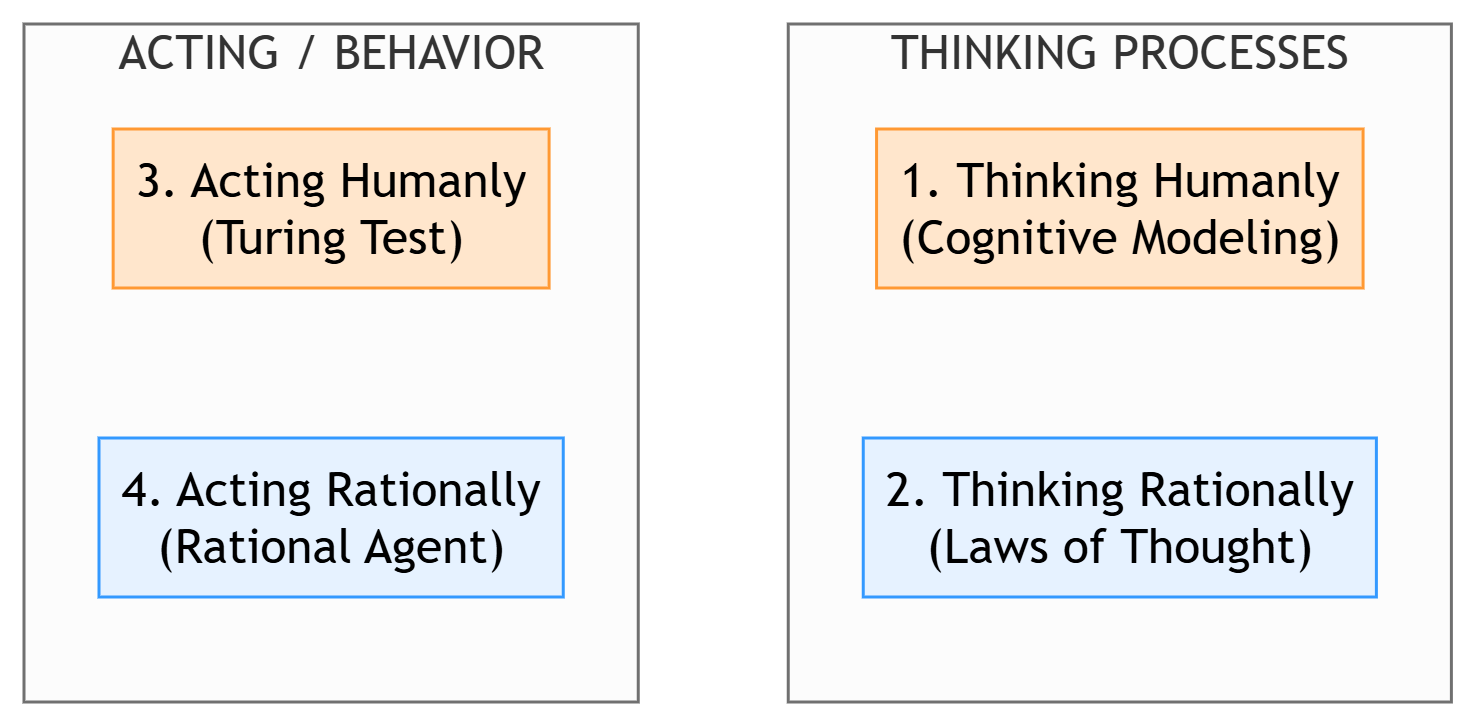
\includegraphics[width=0.75\textwidth,height=0.32\textheight,keepaspectratio]{../Images/chapter_01/four_ai_approaches.png}
\caption{Four Conceptual Approaches to AI Matrix}
\end{figure}

\subsubsection{Detailed Comparison of the Four Views:}

\begin{table}[H]
\centering
\begin{tabular}{|p{\dimexpr 0.2\textwidth - 2\tabcolsep - 1.5\arrayrulewidth\relax}|p{\dimexpr 0.4\textwidth - 2\tabcolsep - 1.5\arrayrulewidth\relax}|p{\dimexpr 0.4\textwidth - 2\tabcolsep - 1.5\arrayrulewidth\relax}|}
\hline
Conceptual Approach & Core Philosophy / Focus & Methodology \& Realization \\
\hline
\textbf{1. Thinking Humanly} & Focuses on mimicking the inner mental processing and cognitive activities of the human brain. & Implemented via \textbf{Cognitive Science} and neuroimaging. Systems are tested by comparing their decision steps to human experimental data. \\
\hline
\textbf{2. Thinking Rationally} & Focuses on using formal logic and the mathematical laws of thought to achieve "correct" reasoning. & Uses \textbf{Propositional/First-Order Logic} and syllogisms (e.g., "If A implies B, and A is true, then B is true"). \\
\hline
\textbf{3. Acting Humanly} & Focuses on creating machines that perform physical and cognitive actions indistinguishable from a human. & Evaluated via the \textbf{Turing Test}. The system's inner logic is irrelevant; only the external, observable behavior matters. \\
\hline
\textbf{4. Acting Rationally} & Focuses on building \textbf{Rational Agents} that act to achieve the best possible outcome (or best expected outcome under uncertainty). & Realized through decision theory, search algorithms, and control theory. This is the \textbf{standard modern view} of AI. \\
\hline
\end{tabular}
\end{table}


\section{Section 2: The Turing Test Benchmark (Q1.2)}

\subsection{1. Definition and Setup}
Introduced by \textbf{Alan Turing} in 1950, the \textbf{Turing Test} (originally the \textit{Imitation Game}) is an operational test of machine intelligence. 

\begin{itemize}
  \item   \textbf{Setup:} A human interrogator communicates with one human and one computer via typed text terminals in separate rooms.
  \item   \textbf{Success Criterion:} If the interrogator cannot reliably tell the computer apart from the human after 5 minutes of questioning, the machine passes the test.
\end{itemize}

\begin{figure}[H]
\centering
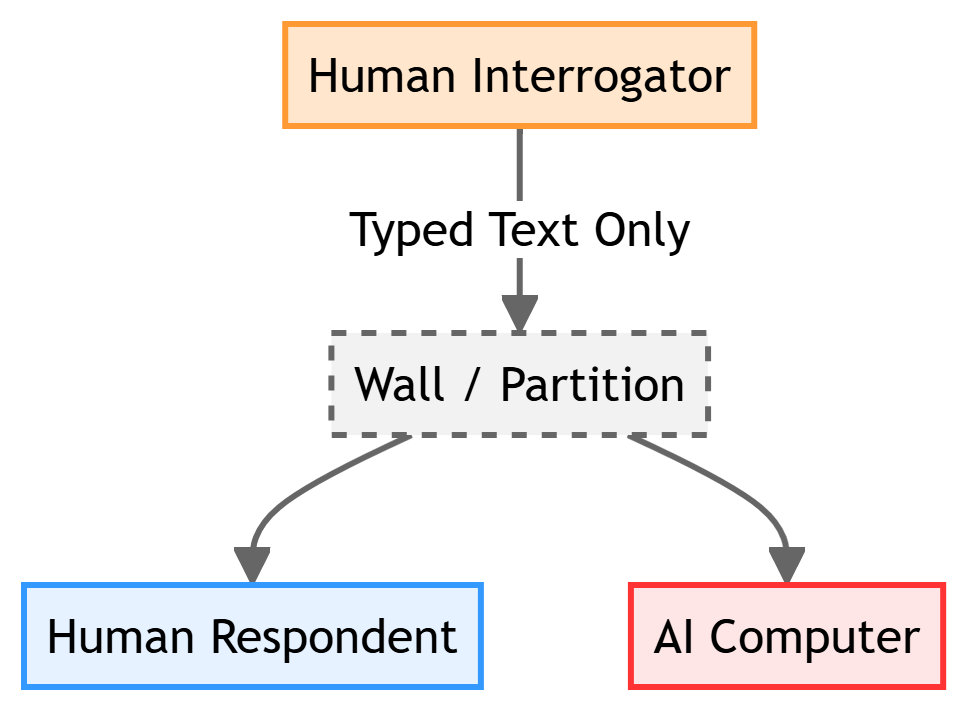
\includegraphics[width=0.75\textwidth,height=0.32\textheight,keepaspectratio]{../Images/chapter_01/turing_test_setup.png}
\caption{Turing Test Setup}
\end{figure}

\subsection{2. Six Key Capabilities Required to Pass the Test}
To pass the Turing Test, a machine must possess the following six primary sub-fields of AI:

\begin{enumerate}
  \item \textbf{Natural Language Processing (NLP):} To communicate successfully in a natural language (like English).
  \item \textbf{Knowledge Representation:} To store facts and beliefs acquired before or during the conversation.
  \item \textbf{Automated Reasoning:} To use stored information to answer questions, draw conclusions, and find logical connections.
  \item \textbf{Machine Learning:} To adapt to new circumstances, detect patterns, and learn from experience.
  \item \textbf{Computer Vision} \textit{(Total Turing Test requirement)}: To perceive physical objects and actions of the interrogator.
  \item \textbf{Robotics} \textit{(Total Turing Test requirement)}: To physically move, interact with, and manipulate the physical environment.
\end{enumerate}


\section{Section 3: Foundational Disciplines of AI (Q1.3)}

Artificial Intelligence is a highly interdisciplinary field. The major contributing disciplines include:

\begin{enumerate}
  \item \textbf{Philosophy (400 BC -- Present):}
\end{enumerate}
    \textit{   }Contribution:* Formulated the ideas that the mind is like a machine, that knowledge is represented in formal languages, and that logical rules can be used to derive conclusions.
\begin{enumerate}
  \item \textbf{Mathematics (c. 800 -- Present):}
\end{enumerate}
    \textit{   }Contribution:* Provided the tools of \textbf{formal logic} (Boolean algebra), \textbf{probability theory} (handling uncertainty), and \textbf{algorithms} (computation limits and tractability).
\begin{enumerate}
  \item \textbf{Economics (1776 -- Present):}
\end{enumerate}
    \textit{   }Contribution:* Contributed utility theory, decision theory, and game theory, which govern how a rational agent makes choices to maximize its expected payoff.
\begin{enumerate}
  \item \textbf{Neuroscience (1861 -- Present):}
\end{enumerate}
    \textit{   }Contribution:* Mapped out how the physical brain processes information, laying the biological foundation for \textbf{Artificial Neural Networks (ANNs)}.
\begin{enumerate}
  \item \textbf{Psychology / Cognitive Science (1879 -- Present):}
\end{enumerate}
    \textit{   }Contribution:* Provided cognitive models to understand how humans think, perceive, and act, guiding the design of human-centric AI systems.
\begin{enumerate}
  \item \textbf{Control Theory \& Cybernetics (1948 -- Present):}
\end{enumerate}
    \textit{   }Contribution:* Contributed feedback loops and the mathematical models to design adaptive, self-regulating systems (e.g., PID controllers, homeostatic systems).


\section{Section 4: Components and Sub-fields of AI (Q1.4)}

\subsection{1. Functional Sub-fields of AI}
AI is comprised of several interacting components, each addressing a specific dimension of intelligence:

\begin{figure}[H]
\centering
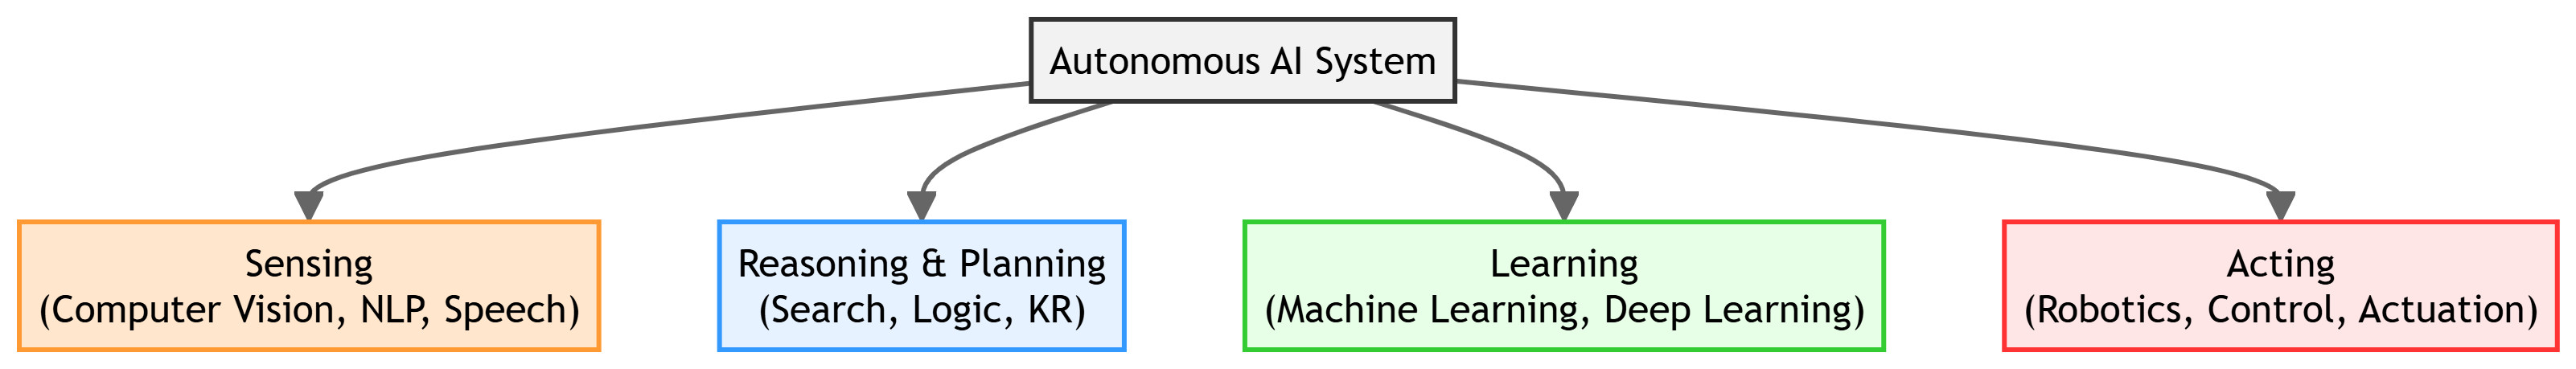
\includegraphics[width=0.75\textwidth,height=0.32\textheight,keepaspectratio]{../Images/chapter_01/ai_components.png}
\caption{Functional Sub-fields/Components of AI}
\end{figure}

\begin{itemize}
  \item   \textbf{Computer Vision:} Enables machines to extract, process, and understand structured information from digital images or videos.
  \item   \textbf{Natural Language Processing (NLP):} Enables computers to process, analyze, and synthesize human languages (syntax, semantics, and pragmatics).
  \item   \textbf{Machine Learning (ML):} The core engine that allows algorithms to improve their performance automatically on a task through exposure to training data.
  \item   \textbf{Expert Systems:} Specialized software systems that emulate the decision-making ability of a human expert in a narrow domain.
  \item   \textbf{Automated Planning \& Decision Making:} Search and logical reasoning systems designed to select sequences of actions to reach a desired goal state.
  \item   \textbf{Robotics:} Integrates vision, control theory, and machine learning to build physical machines that can manipulate objects and navigate environments autonomously.
\end{itemize}


\section{Section 5: Expert Systems (Q1.5)}

\subsection{1. Definition}
An \textbf{Expert System (ES)} is an interactive, computer-based decision-making system that uses knowledge and inference procedures to solve complex, domain-specific problems that typically require human expertise (e.g., medical diagnosis, financial analysis, mineral exploration).

\subsection{2. Detailed Architecture of an Expert System}
A standard Expert System consists of three main non-overlapping components:

\begin{figure}[H]
\centering
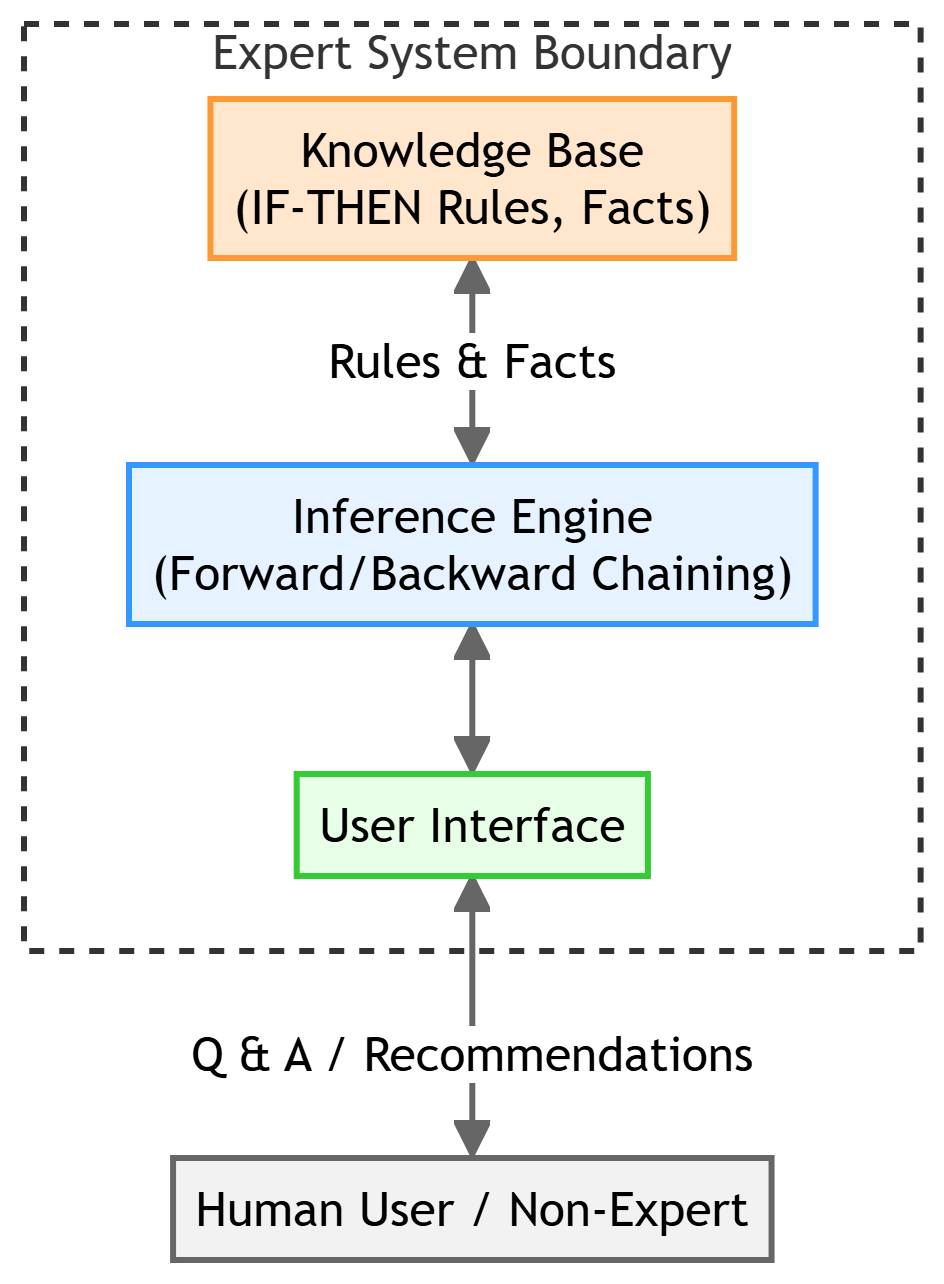
\includegraphics[width=0.75\textwidth,height=0.32\textheight,keepaspectratio]{../Images/chapter_01/expert_system_arch.png}
\caption{Expert System Architecture}
\end{figure}

\subsubsection{Core Components Explained:}
\begin{enumerate}
  \item \textbf{Knowledge Base (KB):} The warehouse of high-quality domain-specific facts, rules, and heuristics compiled from human experts. Information is typically stored in the form of \textbf{IF-THEN production rules}.
  \item \textbf{Inference Engine:} The processing engine that applies logical rules to the Knowledge Base to deduce new information or solve the user's query. It operates in two main modes:
\end{enumerate}
\begin{itemize}
  \item   \textbf{Forward Chaining (Data-Driven):} Starts with known facts and applies rules to infer new facts (reaches a conclusion).
  \item   \textbf{Backward Chaining (Goal-Driven):} Starts with a goal or hypothesis and works backward to find supporting facts.
\end{itemize}
\begin{enumerate}
  \item \textbf{User Interface:} The communication interface that allows a non-expert user to input queries, view recommendations, and inspect the system's reasoning path (via an \textbf{Explanation Facility}).
\end{enumerate}

\subsection{3. Advantages and Disadvantages of Expert Systems}

\subsubsection{Advantages (At least 5 points):}
\begin{enumerate}
  \item \textbf{High Availability:} Expert knowledge is accessible 24/7 on ordinary computer systems, removing dependency on scarce human experts.
  \item \textbf{Consistency:} Does not suffer from fatigue, emotional stress, or cognitive bias; always applies rules uniformly.
  \item \textbf{Speed \& Efficiency:} Processes large volumes of complex, rule-based data in milliseconds, reducing diagnosis or lookup times.
  \item \textbf{Preservation of Expertise:} Captures and preserves the invaluable knowledge of senior experts before they retire or leave an organization.
  \item \textbf{Explanatory Capability:} The system can explicitly print out its exact step-by-step reasoning path (Why/How a conclusion was reached), increasing user trust.
\end{enumerate}

\subsubsection{Disadvantages (At least 5 points):}
\begin{enumerate}
  \item \textbf{Lack of Common Sense:} Completely lacks general, everyday common-sense knowledge; cannot adapt if a problem falls slightly outside its narrow domain.
  \item \textbf{High Maintenance Costs:} Domain knowledge changes over time, requiring expensive manual updates and validation of the rules database.
  \item \textbf{Knowledge Acquisition Bottleneck:} Extracting tacit knowledge from human experts and translating it into rigid IF-THEN rules is extremely slow and difficult.
  \item \textbf{Inability to Learn Automatically:} Unlike modern machine learning systems, traditional expert systems cannot learn from new experiences; rules must be coded manually.
  \item \textbf{Brittleness:} If rules in the Knowledge Base contain contradictions or gaps, the system may crash or produce highly incorrect recommendations without warning.
\end{enumerate}
